
\documentclass[a4paper,UKenglish,cleveref, autoref, thm-restate]{lipics-v2021}

\usepackage[ruled,vlined,linesnumbered]{algorithm2e}
\usepackage{tikz}
\usetikzlibrary{positioning}

\newcommand{\br}[1]{\mathopen{}\left( #1 \right)}
\newcommand{\brc}[1]{\mathopen{}\left\{ #1 \right\}}
\newcommand{\spr}[1]{\mathopen{}\left| #1 \right|}
\newcommand{\fl}[1]{\mathopen{}\left\lfloor #1 \right\rfloor}
\newcommand{\cl}[1]{\mathopen{}\left\lceil #1 \right\rceil}
\newcommand{\angl}[1]{\mathopen{}\langle #1 \rangle}
\newcommand{\e}[1]{\exp\left\{ #1 \right\}}
\newcommand{\diam}{\operatorname{diam}}
\newcommand{\NPcomplete}{\textnormal{$\mathcal{NP}$-Complete}}
\newcommand{\NPhard}{\textnormal{$\mathcal{NP}$-Hard}}
\newcommand{\Cent}{\texttt{Cent}}
\newcommand{\APP}{\texttt{APP}}
\newcommand{\OPT}{\texttt{OPT}}
\newcommand{\COST}{\texttt{COST}}
\newcommand{\argmin}{\operatorname*{argmin}}
\newcommand{\argmax}{\operatorname*{argmax}}

%This is a template for producing LIPIcs articles. 
%See lipics-v2021-authors-guidelines.pdf for further information.
%for A4 paper format use option "a4paper", for US-letter use option "letterpaper"
%for british hyphenation rules use option "UKenglish", for american hyphenation rules use option "USenglish"
%for section-numbered lemmas etc., use "numberwithinsect"
%for enabling cleveref support, use "cleveref"
%for enabling autoref support, use "autoref"
%for anonymousing the authors (e.g. for double-blind review), add "anonymous"
%for enabling thm-restate support, use "thm-restate"
%for enabling a two-column layout for the author/affilation part (only applicable for > 6 authors), use "authorcolumns"
%for producing a PDF according the PDF/A standard, add "pdfa"

%\pdfoutput=1 %uncomment to ensure pdflatex processing (mandatatory e.g. to submit to arXiv)
%\hideLIPIcs  %uncomment to remove references to LIPIcs series (logo, DOI, ...), e.g. when preparing a pre-final version to be uploaded to arXiv or another public repository

%\graphicspath{{./graphics/}}%helpful if your graphic files are in another directory

\bibliographystyle{plainurl}% the mandatory bibstyle

\title{Logarithmic Approximation for Covering Multi-Interface Networks} %TODO Please add

%\titlerunning{Dummy short title} %TODO optional, please use if title is longer than one line

\author{Michał {Szyfelbein}}{Gdańsk University of Technology, Poland}{johnqpublic@dummyuni.org}{https://orcid.org/0000-0002-1825-0097}{}%TODO mandatory, please use full name; only 1 author per \author macro; first two parameters are mandatory, other parameters can be empty. Please provide at least the name of the affiliation and the country. The full address is optional. Use additional curly braces to indicate the correct name splitting when the last name consists of multiple name parts.

% \author{Joan R. Public\footnote{Optional footnote, e.g. to mark corresponding author}}{Department of Informatics, Dummy College, [optional: Address], Country}{joanrpublic@dummycollege.org}{[orcid]}{[funding]}

\authorrunning{M. Szyfelbein} %TODO mandatory. First: Use abbreviated first/middle names. Second (only in severe cases): Use first author plus 'et al.'

\Copyright{Michał Szyfelbein} %TODO mandatory, please use full first names. LIPIcs license is "CC-BY";  http://creativecommons.org/licenses/by/3.0/

\ccsdesc[100]{\textcolor{red}{Replace ccsdesc macro with valid one}} %TODO mandatory: Please choose ACM 2012 classifications from https://dl.acm.org/ccs/ccs_flat.cfm 

\keywords{Dummy keyword} %TODO mandatory; please add comma-separated list of keywords

\category{} %optional, e.g. invited paper

\relatedversion{} %optional, e.g. full version hosted on arXiv, HAL, or other respository/website
%\relatedversiondetails[linktext={opt. text shown instead of the URL}, cite=DBLP:books/mk/GrayR93]{Classification (e.g. Full Version, Extended Version, Previous Version}{URL to related version} %linktext and cite are optional

%\supplement{}%optional, e.g. related research data, source code, ... hosted on a repository like zenodo, figshare, GitHub, ...
%\supplementdetails[linktext={opt. text shown instead of the URL}, cite=DBLP:books/mk/GrayR93, subcategory={Description, Subcategory}, swhid={Software Heritage Identifier}]{General Classification (e.g. Software, Dataset, Model, ...)}{URL to related version} %linktext, cite, and subcategory are optional

%\funding{(Optional) general funding statement \dots}%optional, to capture a funding statement, which applies to all authors. Please enter author specific funding statements as fifth argument of the \author macro.

\acknowledgements{I want to thank \dots}%optional

%\nolinenumbers %uncomment to disable line numbering



%Editor-only macros:: begin (do not touch as author)%%%%%%%%%%%%%%%%%%%%%%%%%%%%%%%%%%
\EventEditors{John Q. Open and Joan R. Access}
\EventNoEds{2}
\EventLongTitle{42nd Conference on Very Important Topics (CVIT 2016)}
\EventShortTitle{CVIT 2016}
\EventAcronym{CVIT}
\EventYear{2016}
\EventDate{December 24--27, 2016}
\EventLocation{Little Whinging, United Kingdom}
\EventLogo{}
\SeriesVolume{42}
\ArticleNo{23}
%%%%%%%%%%%%%%%%%%%%%%%%%%%%%%%%%%%%%%%%%%%%%%%%%%%%%%

\begin{document}

\maketitle

%TODO mandatory: add short abstract of the document
\begin{abstract}
We consider the problem of covering/connecting a multi-interface network with a minimum cost assignment of interfaces to vertices. In the covering problem we demand that every edge is covered by at least one common interface assigned to its endpoints. In the connecting problem we demand that the subgraph induced by each covered edge is connected. 
We give an $O\br{\log m}$ approximation algorithm for both min-sum and min-max versions of the covering/connecting problems. The algorithm is based on rounding the optimal solution of a natural, set-cover-style linear programming relaxation of the problem. We also show how to use this LP to obtain a $k$-approximation algorithm for both problems, where $k$ is the number of interfaces. Importantly, all of the aforementioned procedures work even for the non uniform cost case, when the cost of activating an interface depends on the interface as well as the vertex to which it is assigned.
This improves the previously best known approximation algorithms for the min-max version of the covering problem including: $O\br{\br{1+b}\cdot\br{\ln \Delta+c_{\text{max}}}}$-approximation algorithm, where $b$ is a certain parameter of the input instance which can be as large as $\Omega\br{n}$ and $c_{\text{max}}$ is the maximum cost of activating an interface and $O\br{k}$-approximation algorithm for the uniform cost case \cite{MinimizeTheMaximumDutyInMultiInterfaceNetworks}.

Moreover, we also give combinatorial $O\br{\Delta}$-approximation algorithms for the covering problem with both criterions, thus improving on the previously known $O\br{\Delta\cdot c_{\text{max}}}$ for the min-max version of the problem. We complement these results by showing that the min-sum version of the problem cannot be approximated within a factor of $o\br{\log \Delta}$ on bipartite graphs with uniform costs and on trees with non uniform costs, unless $P=NP$.
\end{abstract}
\section{Introduction}
Designing Internet of Things (IoT) networks often demands establishing connection between large number of devices, which can be achieved by using multiple interfaces at each device. Moreover, the devices present in the network may vary according to the interfaces which can be used. For example some device may be able to use Bluetooth and Wi-Fi, while the others may have Zigbee and Z-Wave interfaces. Since IoT devices are typically resource-constrained, it may be desirable to try to establish every relevant connection, while minimizing the amount of resources required to do so. 

\begin{figure}[t]
\centering
\begin{minipage}[t]{0.49\linewidth}
\centering
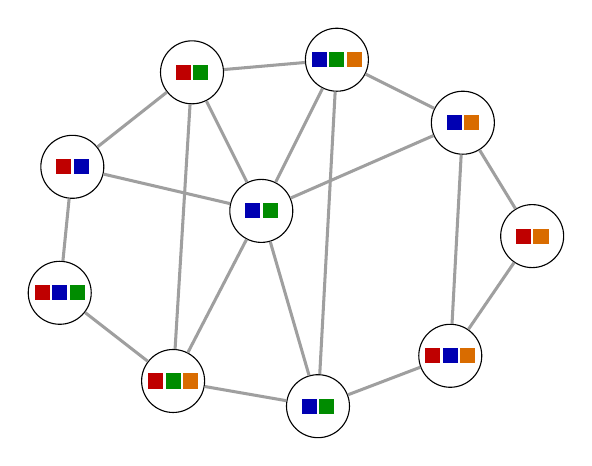
\begin{tikzpicture}[scale=0.80]
    \colorlet{iface1}{red!75!black}
    \colorlet{iface2}{blue!70!black}
    \colorlet{iface3}{green!55!black}
    \colorlet{iface4}{orange!85!black}

    % vertices
    \node[circle, draw, minimum size=8mm, inner sep=0pt] (v1) at (0.0,1.2) {};
    \node[circle, draw, minimum size=8mm, inner sep=0pt] (v2) at (1.9,2.7) {};
    \node[circle, draw, minimum size=8mm, inner sep=0pt] (v3) at (4.2,2.9) {};
    \node[circle, draw, minimum size=8mm, inner sep=0pt] (v4) at (6.2,1.9) {};
    \node[circle, draw, minimum size=8mm, inner sep=0pt] (v5) at (7.3,0.1) {};
    \node[circle, draw, minimum size=8mm, inner sep=0pt] (v6) at (6.0,-1.8) {};
    \node[circle, draw, minimum size=8mm, inner sep=0pt] (v7) at (3.9,-2.6) {};
    \node[circle, draw, minimum size=8mm, inner sep=0pt] (v8) at (1.6,-2.2) {};
    \node[circle, draw, minimum size=8mm, inner sep=0pt] (v9) at (-0.2,-0.8) {};
    \node[circle, draw, minimum size=8mm, inner sep=0pt] (v10) at (3.0,0.5) {};

    % edges
    \draw[gray!75, line width=1.1pt] (v1) -- (v2) -- (v3) -- (v4) -- (v5) -- (v6) -- (v7) -- (v8) -- (v9) -- (v1);
    \draw[gray!75, line width=1.1pt] (v1) -- (v10);
    \draw[gray!75, line width=1.1pt] (v2) -- (v10);
    \draw[gray!75, line width=1.1pt] (v3) -- (v10);
    \draw[gray!75, line width=1.1pt] (v4) -- (v10);
    \draw[gray!75, line width=1.1pt] (v7) -- (v10);
    \draw[gray!75, line width=1.1pt] (v8) -- (v10);
    \draw[gray!75, line width=1.1pt] (v2) -- (v8);
    \draw[gray!75, line width=1.1pt] (v3) -- (v7);
    \draw[gray!75, line width=1.1pt] (v4) -- (v6);

    % available label rectangles in nodes
    \begin{scope}[shift={(v1.center)}]
        \fill[iface1] (-0.26,-0.12) rectangle (-0.02,0.12);
        \fill[iface2] (0.02,-0.12) rectangle (0.26,0.12);
    \end{scope}
    \begin{scope}[shift={(v2.center)}]
        \fill[iface1] (-0.26,-0.12) rectangle (-0.02,0.12);
        \fill[iface3] (0.02,-0.12) rectangle (0.26,0.12);
    \end{scope}
    \begin{scope}[shift={(v3.center)}]
        \fill[iface2] (-0.40,-0.12) rectangle (-0.16,0.12);
        \fill[iface3] (-0.12,-0.12) rectangle (0.12,0.12);
        \fill[iface4] (0.16,-0.12) rectangle (0.40,0.12);
    \end{scope}
    \begin{scope}[shift={(v4.center)}]
        \fill[iface2] (-0.26,-0.12) rectangle (-0.02,0.12);
        \fill[iface4] (0.02,-0.12) rectangle (0.26,0.12);
    \end{scope}
    \begin{scope}[shift={(v5.center)}]
        \fill[iface1] (-0.26,-0.12) rectangle (-0.02,0.12);
        \fill[iface4] (0.02,-0.12) rectangle (0.26,0.12);
    \end{scope}
    \begin{scope}[shift={(v6.center)}]
        \fill[iface1] (-0.40,-0.12) rectangle (-0.16,0.12);
        \fill[iface2] (-0.12,-0.12) rectangle (0.12,0.12);
        \fill[iface4] (0.16,-0.12) rectangle (0.40,0.12);
    \end{scope}
    \begin{scope}[shift={(v7.center)}]
        \fill[iface2] (-0.26,-0.12) rectangle (-0.02,0.12);
        \fill[iface3] (0.02,-0.12) rectangle (0.26,0.12);
    \end{scope}
    \begin{scope}[shift={(v8.center)}]
        \fill[iface1] (-0.40,-0.12) rectangle (-0.16,0.12);
        \fill[iface3] (-0.12,-0.12) rectangle (0.12,0.12);
        \fill[iface4] (0.16,-0.12) rectangle (0.40,0.12);
    \end{scope}
    \begin{scope}[shift={(v9.center)}]
        \fill[iface1] (-0.40,-0.12) rectangle (-0.16,0.12);
        \fill[iface2] (-0.12,-0.12) rectangle (0.12,0.12);
        \fill[iface3] (0.16,-0.12) rectangle (0.40,0.12);
    \end{scope}
    \begin{scope}[shift={(v10.center)}]
        \fill[iface2] (-0.26,-0.12) rectangle (-0.02,0.12);
        \fill[iface3] (0.02,-0.12) rectangle (0.26,0.12);
    \end{scope}
\end{tikzpicture}

\vspace{1mm}
{\scriptsize Available labels}
\end{minipage}
\hfill
\begin{minipage}[t]{0.49\linewidth}
\centering
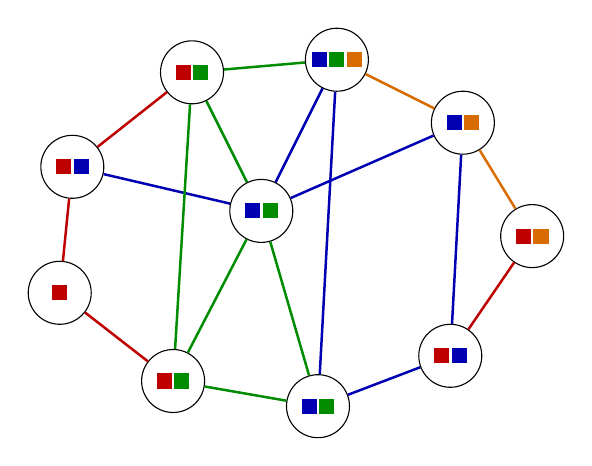
\begin{tikzpicture}[scale=0.80]
    \colorlet{iface1}{red!75!black}
    \colorlet{iface2}{blue!70!black}
    \colorlet{iface3}{green!55!black}
    \colorlet{iface4}{orange!85!black}

    % vertices
    \node[circle, draw, minimum size=8mm, inner sep=0pt] (v1) at (0.0,1.2) {};
    \node[circle, draw, minimum size=8mm, inner sep=0pt] (v2) at (1.9,2.7) {};
    \node[circle, draw, minimum size=8mm, inner sep=0pt] (v3) at (4.2,2.9) {};
    \node[circle, draw, minimum size=8mm, inner sep=0pt] (v4) at (6.2,1.9) {};
    \node[circle, draw, minimum size=8mm, inner sep=0pt] (v5) at (7.3,0.1) {};
    \node[circle, draw, minimum size=8mm, inner sep=0pt] (v6) at (6.0,-1.8) {};
    \node[circle, draw, minimum size=8mm, inner sep=0pt] (v7) at (3.9,-2.6) {};
    \node[circle, draw, minimum size=8mm, inner sep=0pt] (v8) at (1.6,-2.2) {};
    \node[circle, draw, minimum size=8mm, inner sep=0pt] (v9) at (-0.2,-0.8) {};
    \node[circle, draw, minimum size=8mm, inner sep=0pt] (v10) at (3.0,0.5) {};

    % edges colored by covering label
    \draw[iface1, line width=0.9pt] (v1) -- (v2);
    \draw[iface3, line width=0.9pt] (v2) -- (v3);
    \draw[iface4, line width=0.9pt] (v3) -- (v4);
    \draw[iface4, line width=0.9pt] (v4) -- (v5);
    \draw[iface1, line width=0.9pt] (v5) -- (v6);
    \draw[iface2, line width=0.9pt] (v6) -- (v7);
    \draw[iface3, line width=0.9pt] (v7) -- (v8);
    \draw[iface1, line width=0.9pt] (v8) -- (v9);
    \draw[iface1, line width=0.9pt] (v9) -- (v1);
    \draw[iface2, line width=0.9pt] (v1) -- (v10);
    \draw[iface3, line width=0.9pt] (v2) -- (v10);
    \draw[iface2, line width=0.9pt] (v3) -- (v10);
    \draw[iface2, line width=0.9pt] (v4) -- (v10);
    \draw[iface3, line width=0.9pt] (v7) -- (v10);
    \draw[iface3, line width=0.9pt] (v8) -- (v10);
    \draw[iface3, line width=0.9pt] (v2) -- (v8);
    \draw[iface2, line width=0.9pt] (v3) -- (v7);
    \draw[iface2, line width=0.9pt] (v4) -- (v6);

    % selected labels in solution
    \begin{scope}[shift={(v1.center)}]
        \fill[iface1] (-0.26,-0.12) rectangle (-0.02,0.12);
        \fill[iface2] (0.02,-0.12) rectangle (0.26,0.12);
    \end{scope}
    \begin{scope}[shift={(v2.center)}]
        \fill[iface1] (-0.26,-0.12) rectangle (-0.02,0.12);
        \fill[iface3] (0.02,-0.12) rectangle (0.26,0.12);
    \end{scope}
    \begin{scope}[shift={(v3.center)}]
        \fill[iface2] (-0.40,-0.12) rectangle (-0.16,0.12);
        \fill[iface3] (-0.12,-0.12) rectangle (0.12,0.12);
        \fill[iface4] (0.16,-0.12) rectangle (0.40,0.12);
    \end{scope}
    \begin{scope}[shift={(v4.center)}]
        \fill[iface2] (-0.26,-0.12) rectangle (-0.02,0.12);
        \fill[iface4] (0.02,-0.12) rectangle (0.26,0.12);
    \end{scope}
    \begin{scope}[shift={(v5.center)}]
        \fill[iface1] (-0.26,-0.12) rectangle (-0.02,0.12);
        \fill[iface4] (0.02,-0.12) rectangle (0.26,0.12);
    \end{scope}
    \begin{scope}[shift={(v6.center)}]
        \fill[iface1] (-0.26,-0.12) rectangle (-0.02,0.12);
        \fill[iface2] (0.02,-0.12) rectangle (0.26,0.12);
    \end{scope}
    \begin{scope}[shift={(v7.center)}]
        \fill[iface2] (-0.26,-0.12) rectangle (-0.02,0.12);
        \fill[iface3] (0.02,-0.12) rectangle (0.26,0.12);
    \end{scope}
    \begin{scope}[shift={(v8.center)}]
        \fill[iface1] (-0.26,-0.12) rectangle (-0.02,0.12);
        \fill[iface3] (0.02,-0.12) rectangle (0.26,0.12);
    \end{scope}
    \begin{scope}[shift={(v9.center)}]
        \fill[iface1] (-0.12,-0.12) rectangle (0.12,0.12);
    \end{scope}
    \begin{scope}[shift={(v10.center)}]
        \fill[iface2] (-0.26,-0.12) rectangle (-0.02,0.12);
        \fill[iface3] (0.02,-0.12) rectangle (0.26,0.12);
    \end{scope}
\end{tikzpicture}

\vspace{1mm}
{\scriptsize Example covering assignment}
\end{minipage}

\caption{An example instance of a multi-interface network with available interfaces at each vertex and a feasible covering assignment.}
\label{example_solution}
\end{figure}
We model the above problem as one of two graph problems, in which devices are modeled as vertices of a graph. With each vertex we associate a set of labels representing the set of available interfaces. In the covering problem each edge in this graph represents a connection that we wish to establish by assigning a common interface to its endpoints. 
To see an example, see Figure~\ref{example_solution}. In the connection problem each edge represents a connection which is possible to be activated by assigning a common interface to its endpoints, but we only require that the subgraph induced by the activated edges is connected. Additionally, activating a given interface at a given vertex may incur arbitrary cost. The goal is to minimize either the min-max cost (the maximum cost per vertex) or min-sum cost (sum of costs over all vertices). Both problems are NP-hard and cannot be approximated within $O\br{\log \Delta}$-factor unless P=NP.
\subsection{Related Work}
% \subsection{Our contribution and techniques}
% In this paper we give a first $O\br{\log m}$-approximation algorithm for both optimization criterions. This improves the previously known result of [cite] which gave an $O\br{\br{1+b}\cdot\log n}$-approximation algorithm for the min-max version of the problem, where $b$ is a parameter denoting an existence of a $b$-owner function [cite]. Our approach is based on a natural set-cover-like linear relaxation of the problem and a randomized rounding procedure. We also show how to use the same LP relaxation to obtain a $k$-approximation algorithm for both problems, where $k$ is the number of interfaces. Importantly, we allow the cost of function also to depend on the vertex to which the interface is assigned, which is more general than the previously considered cost function dependent only on the interface.

% Then, we shift our attention towards combinatorial algorithms and give a simple $\Delta$-approximation algorithm for the min-sum version of the problem and a $2\Delta$-approximation algorithm for the min-max version of the problem, where $\Delta$ is the maximum degree of the input graph. This improves the previously known $O\br{\Delta\cdot c_{\text{max}}}$-approximation algorithm for the min-max version of the problem, where $c_{\text{max}}$ is the maximum cost of activating an interface.

% Finally, we complement our positive results by showing that the min-sum version of the problem cannot be approximated within a factor of $o\br{\log \Delta}$ on bipartite graphs with uniform costs and on trees with non uniform costs, unless $P=NP$.
\section{Preliminaries}


Let $G=\br{V, E}$ be a connected simple graph. Let $\lambda\colon V \to [k]$ be a function that assigns to each vertex $v\in V$ a set of available interfaces. In the \emph{covering problem} we wish to find an assignment $\lambda_A\colon V \to [k]$ such that $\lambda_A\br{v} \subseteq \lambda\br{v}$ for all $v\in V$ and for every edge $uv\in E$ we have $\lambda_A\br{u} \cap \lambda_A\br{v} \neq \emptyset$. We call such an assignment a \emph{covering assignment}. In the \emph{connection problem} we wish to find an assignment $\lambda_A\colon V \to [k]$ such that $\lambda_A\br{v} \subseteq \lambda\br{v}$ for all $v\in V$ and for every $i\in[k]$ the subgraph of $G$ induced by the edges $uv\in E$, such that $\lambda_A\br{u}\cap\lambda\br{v}\neq\emptyset$. We call such an assignment a \emph{connecting assignment}.

We additionally assume, that a cost function $c\colon [k]\times V \to \mathbb{N}_{\geq 0}$ is given, which denotes the cost of assingining the interface $i\in[k]$ to vertex $v\in V$. The sum cost of the assignment is defined as:
$$\COST_A=\sum_{v\in V}\sum_{i\in\lambda_A\br{v}}c\br{i, v}.$$
The goal of the min-sum assignment problem is to find an assignment $\lambda_A$ that minimizes $\COST_A$.
The max cost of the assignment is defined as:
$$\COST_W=\max_{v\in V}\sum_{i\in\lambda_A\br{v}}c\br{i, v}.$$
The goal of the min-max assignment problem is to find an assignment $\lambda_A$ that minimizes $\COST_W$.
\section{LP based approximation algorithms}

\subsection{ILP formulation of covering multi-interface networks}

Below we show an $O\br{\log m}$ approximation algorithm for both problems. We start with the following ILP formulation of the min-sum covering assignment problem. Let $x_{i, v}$ be a binary variable that is $1$ if and only if the interface $i\in[k]$ is assigned to vertex $v\in V$. Then the min-sum covering assignment problem can be formulated as follows:
\begin{align*}
    \text{min} \quad & \sum_{v\in V}\sum_{i\in\lambda\br{v}}c\br{i, v}\cdot x_{i, v}\\
    \text{s.t.} \quad & \sum_{i\in\lambda\br{u}\cap\lambda\br{v}}\min\brc{x_{i, u}, x_{i, v}} \geq 1 \quad \forall uv\in E\\
    & x_{i, v} \in \{0, 1\} \quad \forall v\in V, i\in\lambda\br{v}
\end{align*}
Similarly, the min-max covering assignment problem can be formulated as follows:
\begin{align*}
    \text{min} \quad & M\\
    \text{s.t.} \quad & \sum_{i\in\lambda\br{v}}x_{i, v}\cdot c\br{i, v} \leq M \quad \forall v\in V\\
    & \sum_{i\in\lambda\br{u}\cap\lambda\br{v}}\min\brc{x_{i, u}, x_{i, v}} \geq 1 \quad \forall uv\in E\\
    & x_{i, v} \in \{0, 1\} \quad \forall v\in V, i\in\lambda\br{v}
\end{align*}

Note that the above formulations are not linear due to the presence of the $\min$ function. However, by adding an additional variable $y_{i, uv}$ we can rewrite the constraint $\sum_{i\in\lambda\br{u}\cap\lambda\br{v}}\min\brc{x_{i, u}, x_{i, v}} \geq 1$ as $\sum_{i\in\lambda\br{u}\cap\lambda\br{v}}y_{i, uv} \geq 1$ together with the constraints $y_{i, uv} \leq x_{i, u}$ and $y_{i, uv} \leq x_{i, v}$ for every $i\in\lambda\br{u}\cap\lambda\br{v}$ and $uv\in E$. Thus, we can solve the LP relaxation of each of the above formulations in polynomial time.
\subsection{Randomized $O\br{\log m}$-approximation algorithm for the covering problem}

\begin{algorithm}[H]
\caption{A relaxation-based $O(\log m)$-approximation algorithm.}
Solve the LP relaxation and obtain an optimal solution $\{x_{i, v}\}_{i\in\lambda(v), v\in V}$.

Pick independent uniformly random thresholds $t_i \in (0, 1)$, for each $i \in [k]$.

Set $\lambda_A(v) = \{i \in \lambda(v) \colon 3\ln m\cdot x_{i, v} \geq t_i\}$, for every $v \in V$.

\Return{$\{\lambda_A(v)\}_{v\in V}$.}
\end{algorithm}

\begin{theorem}
The above algorithm is an $O(\log m)$-approximation algorithm for both the min-sum and the min-max covering assignment problems which succeeds with high probability.
\end{theorem}
\begin{proof}
We have the following lemmas:
\begin{lemma}
    The algorithm returns a solution of cost at most $9\ln m \cdot \OPT$ with high probability.
\end{lemma}
\begin{proof}
By $X_{v, i}$ denote the indicator random variable that is $1$ if $x_{i, v} \geq t_i$ and $0$ otherwise. Then we can write $c\br{\lambda_A\br{v}} = \sum_{i\in\lambda\br{v}}X_{v, i}\cdot c\br{i, v}$. We have: $\mathbb{E}[X_{v, i}] = \Pr[i \in \lambda_A\br{v}] = 3\ln m\cdot x_{i, v}$. Thus, $\mathbb{E}[c\br{\lambda_A\br{v}}] = 3\ln m \cdot \sum_{i\in\lambda\br{v}}x_{i, v}\cdot c\br{i, v}$. By applying the Chernoff bound with $\delta = 2$ we get that 
\begin{align*}
    \Pr[c\br{\lambda_A\br{v}} \geq 3\cdot \mathbb{E}[c\br{\lambda_A\br{v}}]] & 
    \leq \br{\frac{e^2}{9}}^{\mathbb{E}[c\br{\lambda_A\br{v}}]}
    \leq \e{-\mathbb{E}[c\br{\lambda_A\br{v}}]}\leq \frac{1}{m^3}
\end{align*}
where the last inequality is by using the fact that trivially, $\sum_{i\in\lambda\br{v}}x_{i, v}\cdot c\br{i, v} \geq 1$ for all $v \in V$. If otherwise, then $v$ would have no neighbors which contradicts connectivity. By applying the union bound over all $n$ vertices we get that with probability at least $1-\frac{n}{m^3}\geq 1-\frac{1}{m^2}$ for every $v\in V$, $c\br{\lambda_A\br{v}} \leq 9\ln m \cdot \sum_{i\in\lambda\br{v}}x_{i, v}\cdot c\br{i, v}$. Thus, depending on the cost function, with high probability we have $\COST_A \leq 9\ln m \cdot \sum_{v\in V}\sum_{i\in\lambda\br{v}}x_{i, v}\cdot c\br{i, v} = 9\ln m \cdot \OPT$ or $\COST_W \leq 9\ln m \cdot \max_{v\in V}\sum_{i\in\lambda\br{v}}x_{i, v}\cdot c\br{i, v} = 9\ln m \cdot \OPT$. 
\end{proof}

    \begin{lemma}
With high probability, the above algorithm returns a covering assignment.
    \end{lemma}
\begin{proof}
    Consider an edge $uv\in E$. We have:
\begin{align*}
    \Pr[\lambda_A\br{u}\cap\lambda_A\br{v}=\emptyset] & = \prod_{i\in\lambda\br{u}\cap\lambda\br{v}}\Pr[t_i > \min\brc{x_{i, u}, x_{i, v}}]\\
    & = \prod_{i\in\lambda\br{u}\cap\lambda\br{v}}\brc{1-3\ln m \cdot\min\brc{x_{i, u}, x_{i, v}}}\\&
    \leq \prod_{i\in\lambda\br{u}\cap\lambda\br{v}}\e{-3\ln m \cdot\min\brc{x_{i, u}, x_{i, v}}} 
    \\& = \e{-3\ln m \cdot\sum_{i\in\lambda\br{u}\cap\lambda\br{v}}\min\brc{x_{i, u}, x_{i, v}}}\\
    & \leq \e{-3\ln m} = \frac{1}{m^3}
\end{align*}
By applying the union bound over all $m$ edges we get that the algorithm returns a covering assignment with probability at least $1-\frac{1}{m^2}$.
\end{proof}
Combining the above lemmas gives the claim.
\end{proof}
\subsection{A $k$-approximation algorithm for the covering problem}

\begin{algorithm}[H]
\caption{A relaxation-based $k$-approximation algorithm.}
Solve the LP relaxation and obtain an optimal solution $\{x_{i, v}\}_{i\in\lambda(v), v\in V}$.

Set $\lambda_A(v) = \{i \in \lambda(v) : x_{i, v} \geq \frac{1}{k}\}$, for every $v \in V$.

\Return{$\{\lambda_A(v)\}_{v\in V}$.}
\end{algorithm}
\begin{theorem}
The above algorithm is a $k$-approximation algorithm for both the min-sum and the min-max covering assignment problems.
\end{theorem}
\begin{proof}
Consider an edge $uv\in E$. By averaging, there exists and interface $i\in\lambda\br{u}\cap\lambda\br{v}$ such that $\min\brc{x_{i, u}, x_{i, v}} \geq \frac{1}{k}$. Thus, $i\in\lambda_A\br{u}\cap\lambda_A\br{v}$ and the algorithm returns a covering assignment. Moreover, since $x_{i, v} \geq \frac{1}{k}$ for every $i\in\lambda_A\br{v}$, we have that $c\br{\lambda_A\br{v}} = \sum_{i\in\lambda_A\br{v}}c\br{i, v} \leq k \cdot \sum_{i\in\lambda_A\br{v}}x_{i, v}\cdot c\br{i, v}$. Thus, depending on the cost function, we have $\COST_A \leq k \cdot \sum_{v\in V}\sum_{i\in\lambda\br{v}}x_{i, v}\cdot c\br{i, v} = k \cdot \OPT$ or $\COST_W \leq k \cdot \max_{v\in V}\sum_{i\in\lambda\br{v}}x_{i, v}\cdot c\br{i, v} = k \cdot \OPT$.
\end{proof}
\subsection{ILP formulation for the connection problem}
We use a similar LP to model the connection problem, however we use additional flow variables to encode the connectivity requirement. The $x_{i, v}$ variables are defined as before. For each edge $e$ we add additional flow variable $y_{e}$ which is $1$ if and only if the edge $e$ is covered by the solution. Then we can formulate the min-sum connection problem as follows:
\begin{align*}
    \text{min} \quad & \sum_{v\in V}\sum_{i\in\lambda\br{v}}c\br{i, v}\cdot x_{i, v}\\
    \text{s.t.} \quad & \sum_{i\in\lambda\br{u}\cap\lambda\br{v}}\min\brc{x_{i, u}, x_{i, v}} \geq y_{uv} \quad \forall uv\in E\\
    & y\br{\delta\br{S}}\geq 1 \quad \forall S\subset V\\
    & x_{i, v}  \in \{0, 1\} \quad \forall v\in V, i\in\lambda\br{v}\\
    & y_{uv} \in \{0, 1\} \quad \forall uv\in E
\end{align*}

Similarly, the min-max connection problem can be formulated as follows:
\begin{align*}
    \text{min} \quad & M\\
    \text{s.t.} \quad & \sum_{i\in\lambda\br{v}}x_{i, v}\cdot c\br{i, v} \leq M \quad \forall v\in V\\
    & \sum_{i\in\lambda\br{u}\cap\lambda\br{v}}\min\brc{x_{i, u}, x_{i, v}} \geq y_{uv} \quad \forall uv\in E\\
    & y\br{\delta\br{S}}\geq 1 \quad \forall S\subset V\\
    & x_{i, v}  \in \{0, 1\} \quad \forall v\in V, i\in\lambda\br{v}\\
    & y_{uv} \in \{0, 1\} \quad \forall uv\in E
\end{align*}
    
Observe that both of the above ILPs have exponential number of constraints, but we can solve their LP relaxations in polynomial time by using the ellipsoid method and a separation oracle for the cut constraints, which can be implemented by using a max-flow algorithm. 
\begin{theorem}
    There exists an $O\br{\log m}$-approximation algorithm for both the min-sum and the min-max connection assignment problems which succeeds with high probability.
\end{theorem}
\begin{proof}
    We show that the algorithm for the covering problem described in the previous section can be used to obtain an $O\br{\log m}$-approximation algorithm for the connection problem. Observe that the aformentioned procedure basically, scales-up all of the values of $x_{i,v}$ by a factor of $3\ln m$ and then applies the same randomized rounding procedure. Let $\bar{\mathbf{x}}$ and $\bar{\mathbf{y}}$ both be vectors obtained by scaling $\mathbf{x}$ and $\mathbf{y}$ in this manner. It is easy to see that this is a valid LP solution. By applying the previous argument we see that the cost of such a solution is at most $O\br{\log m}\cdot\OPT$. We now show the following lemma:
    \begin{lemma}
        Assign a value $y_e = 1$ with probabilty $\bar{y_e}$ and $y_e = 0$ otherwise.
        Then, with high probability, the subgraph $H$ induced by the edges $e$ such that $y_e \geq 1$ is connected.
    \end{lemma}
    \begin{proof}
        Fix any $S\subset V$. Let $k\in\mathbb{N}$, such that $k\leq y\br{\delta\br{S}}<k+1$.
        We have:
        \begin{align*}
            \Pr[\spr{\delta\br{S}}=0] & = \prod_{e\in\delta\br{S}}\Pr[y_e=0] = \prod_{e\in\delta\br{S}}(1-\bar{y_e}) \\&\leq \prod_{e\in\delta\br{S}}\e{-\bar{y_e}} = \e{-\bar{y}\br{\delta\br{S}}} \leq \e{-3k\ln m} = \frac{1}{m^{3k}}
        \end{align*}
        
        A cut in $G$ is called an $\alpha$-minimum cut if its value is less than $\alpha$ times the value of a minimum cut in $G$. 
        We now make a use of the Karger's property \cite{MinimumCutsInNearLinearTime}:
        \begin{lemma}[Karger's property]
            Let $G$ be a graph. The number of $\alpha$-minimum cuts in $G$ is at most $n^{2\alpha}$.
        \end{lemma}
        Observe that by construction of the LP, every fractional cut has a value of at least $1$ so there are at most $n^{2k}$ cuts of value less than $k$. By applying the union bound we get that:
\begin{align*}
    \Pr[\exists S\subset V\colon \spr{\delta\br{S}}=0] & \leq \sum_{k=1}^{\infty}\sum_{\substack{S\subset V\\y\br{\delta\br{S}}<k+1}}\Pr[\spr{\delta\br{S}}=0] \\&\leq \sum_{k=1}^{\infty}n^{2k}\cdot \frac{1}{m^{3k}} = \sum_{k=1}^{\infty}\frac{1}{m^k} = \frac{1}{m-1}
\end{align*}
Thus, with high probability, $H$ is connected.
\end{proof}

Therefore, since $H$ is connected we can reuse the argument from the previous section to show that performing the randomized rounding procedure on the solution $\bar{\mathbf{x}}$ gives us a covering assignment for $H$ of cost at most $O\br{\log m}\cdot\OPT$ with high probability. Since a covering assignment of a spanning subgraph is a connecting assignment of the orginal graph the claim follows.
\end{proof}
\section{Combinatorial $O\br{\Delta}$-approximation algorithms}
\subsection{$\Delta$-approximation for the min-sum covering problem}
\begin{algorithm}[H]
\caption{A simple $\Delta$-approximation algorithm for the min-sum covering problem.}
Initialize $\lambda_A(v) = \emptyset$ for every $v \in V$.

For every edge $uv\in E$, let $i_{uv}=\argmin_{j\in\lambda\br{u}\cap\lambda\br{v}}\brc{c\br{j, u}+c\br{j, v}}$. 
Set $\lambda_A\br{u} = \lambda_A\br{u} \cup \{i_{uv}\}$ and $\lambda_A\br{v} = \lambda_A\br{v} \cup \{i_{uv}\}$.

\Return{$\{\lambda_A(v)\}_{v\in V}$.}
\end{algorithm}
\begin{theorem}
    The above algorithm is a $\Delta$-approximation algorithm for the min-sum covering problem.
\end{theorem}
\begin{proof}
    Consider any optimal solution $\lambda_A^*$. For any edge $uv\in E$, let $i_{uv}^* \in \lambda_A^*\br{u}\cap\lambda_A^*\br{v}$ be any interface that covers $uv$ in the optimal solution.
    For every vertex $v\in V$ and edge $uv\in E$ incident to $v$, we say that $v$ dominates $uv$, if $c\br{i_{uv}^*, v} \geq c\br{i_{uv}^*, u}$ (with ties broken arbitrarily). Let $D\br{v}$ be the set of edges dominated by $v$. We have the following inequality:
    $$
    \OPT \geq \sum_{v\in V}\max_{uv\in D\br{v}}\brc{c\br{i_{uv}^*, u}+c\br{i_{uv}^*, v}}.
    $$
    The cost of the solution built by the procedure is upper bounded by:
    \begin{align*}
        \sum_{uv\in E}\min_{i\in \lambda\br{u}\cap\lambda\br{v}} \brc{c\br{i, u}+c\br{i, v}} &=\sum_{v\in V}\sum_{uv\in D\br{v}}\min_{i\in \lambda\br{u}\cap\lambda\br{v}} \brc{c\br{i, u}+c\br{i, v}}
         \\&\leq 
        \sum_{v\in V}\sum_{uv\in D\br{v}} \max_{uv\in D\br{v}}\brc{c\br{i_{uv}^*, u}+c\br{i_{uv}^*, v}} 
        \\&= 
        \sum_{v\in V}\Delta\cdot \max_{uv\in D\br{v}}\brc{c\br{i_{uv}^*, u}+c\br{i_{uv}^*, v}}
        \leq 
        \Delta \cdot \OPT
    \end{align*}
    Since by construction, the solution returned by the procedure is a covering assignment, the claim follows.
\end{proof}
\subsection{$\Delta$-approximation for the min-sum connection problem}
\begin{algorithm}[H]
\caption{A simple $\Delta$-approximation algorithm for the min-sum connection problem.}
Initialize $\lambda_A(v) = \emptyset$ for every $v \in V$.

For every edge $uv\in E$, let $i_{uv}=\argmin_{j\in\lambda\br{u}\cap\lambda\br{v}}\brc{c\br{j, u}+c\br{j, v}}$ and set $c_{uv} = c\br{i_{uv}, u}+c\br{i_{uv}, v}$. 

Let $T$ be a minimum spanning tree of $G$ with respect to the edge weights $c_{uv}$. 

For every edge $uv\in T$, set $\lambda_A\br{u} = \lambda_A\br{u} \cup \{i_{uv}\}$ and $\lambda_A\br{v} = \lambda_A\br{v} \cup \{i_{uv}\}$.

\Return{$\{\lambda_A(v)\}_{v\in V}$.}
\end{algorithm}
\begin{theorem}
    The above algorithm is a $\Delta$-approximation algorithm for the min-sum connection assignment problem.
\end{theorem}
\begin{proof}
    Consider any optimal solution $\lambda_A^*$ and let $G^*$ be the subgraph of $G$ induced by the edges covered in the optimal solution. Let $T^*$ be a spanning tree of $G^*$. For any edge $uv\in E\br{T^*}$, let $i_{uv}^* \in \lambda_A^*\br{u}\cap\lambda_A^*\br{v}$ be any interface that covers $uv$ in $T^*$.
    For every vertex $v\in V$ and edge $uv\in E\br{T^*}$ incident to $v$, we say that $v$ dominates $uv$, if $c\br{i_{uv}^*, v} \geq c\br{i_{uv}^*, u}$ (with ties broken arbitrarily). Let $D\br{v}$ be the set of edges dominated by $v$ in $T^*$. We have the following inequality:
    $$
    \OPT\br{G} = \COST_A\br{T^*} \geq \sum_{v\in V}\max_{uv\in D\br{v}}\brc{c\br{i_{uv}^*, u}+c\br{i_{uv}^*, v}}.
    $$
    The cost of the solution built by the procedure is upper bounded by:
    \begin{align*}
        \sum_{uv\in E\br{T}}\min_{i\in \lambda\br{u}\cap\lambda\br{v}} \brc{c\br{i, u}+c\br{i, v}} &\leq \sum_{uv\in E\br{T^*}}\min_{i\in \lambda\br{u}\cap\lambda\br{v}} \brc{c\br{i, u}+c\br{i, v}}
        \\&=\sum_{v\in V}\sum_{uv\in D\br{v}}\min_{i\in \lambda\br{u}\cap\lambda\br{v}} \brc{c\br{i, u}+c\br{i, v}}
         \\&\leq 
        \sum_{v\in V}\sum_{uv\in D\br{v}} \max_{uv\in D\br{v}}\brc{c\br{i_{uv}^*, u}+c\br{i_{uv}^*, v}} 
        \\&= 
        \sum_{v\in V}\Delta\cdot \max_{uv\in D\br{v}}\brc{c\br{i_{uv}^*, u}+c\br{i_{uv}^*, v}}
        \leq 
        \Delta \cdot \OPT
    \end{align*}
    where the first inequality is by the optimality of $T$.

    Since by construction, the solution returned by the procedure is a covering assignment, the claim follows.
\end{proof}

\subsection{$2\Delta$-approximation for the min-max covering problem}

We start with the following observation. Let $M$ be any matching in $G$. Then, we have $\OPT\geq \max_{uv\in M}\brc{\min_{i\in \lambda\br{u}\cap\lambda\br{v}} \brc{\max\brc{c\br{i, u},c\br{i, v}}}}$. This is due to the fact, that for any edge $uv\in M$ there needs to exist a common interface $i\in \lambda_A\br{u}\cap\lambda_A\br{v}$ in the optimal solution. Since the above expression represents choosing the (localy) best interface for each edge in the matching, it is upper bounded by the cost of the optimal solution. We use the fact, that for any graph, there always exists a matching incident to every vertex of degree $\Delta$, except at most one. We also note that if $G'$ is a subgraph of $G$, then $\OPT\br{G'} \leq \OPT\br{G}$, since any covering assignment for $G$ is also a covering assignment for $G'$.
\begin{algorithm}[H]
\caption{$2\Delta$-approximation algorithm for the min-max covering problem}
If $n=1$ then return $\{\lambda\br{v}=\emptyset\}$, where $v$ is the only vertex in $G$.

Let $M$ be a matching in $G$, which is incident to the largest number of vertices of degree $\Delta$. Let $e=$ be an arbitrary edge incident to the remaining vertex of degree $\Delta$, if it exists. 

For every $H\in G-\br{M\cup\{e\}}$, call the procedure recursively and obtain a covering assignment $\lambda_A$ for all vertices of $H$.

For every edge $uv\in M\cup\{e\}$, let $i_{uv}=\argmin_{i\in\lambda\br{u}\cap\lambda\br{v}}\brc{\max\brc{c\br{i, u}, c\br{i, v}}}$. Set $\lambda_A\br{u} = \lambda_A\br{u} \cup \{i_{uv}\}$ and $\lambda_A\br{v} = \lambda_A\br{v} \cup \{i_{uv}\}$.

\Return{$\{\lambda_A(v)\}_{v\in V}$.}
\end{algorithm}
\begin{theorem}
    The above algorithm is a $2\Delta$-approximation algorithm for the min-max covering assignment problem.
\end{theorem}
\begin{proof}
    By construction, the solution returned by the procedure is a covering assignment. We show that its cost is at most $2\Delta\cdot \OPT$. We claim by induction that this is the case. For $n=1$, i. e., $\Delta=1$, the cost is $0$ and the claim holds. Assume, that the claim holds for some value of $\Delta$.
    By definition of $M$ we get that the cost of the solution is upper bounded by:
\begin{align*}
    &\max_{uv\in M\cup\brc{e}}\brc{\min_{i\in\lambda\br{u}\cap\lambda\br{v}}\brc{\max\brc{c\br{i, u}, c\br{i, v}}}} + \max_{H\in G-\br{M\cup\{e\}}}\COST_W\br{H} \\&\leq 
    2\cdot\OPT\br{G}+ \max_{H\in G-\br{M\cup\{e\}}} \brc{2\cdot\br{\Delta-1}\cdot \OPT\br{H}} \leq 2\Delta\cdot \OPT\br{G}
\end{align*}
where the first inequality is by the fact that $M$ and $\brc{e}$ are both matchings and the induction hypothesis.
\end{proof}
\section{Approximation hardness of covering multi-interface networks}
The reduction are from the Set Cover problem, which is defined as follows. We are given a universe $U$ of $n$ elements and a family $\mathcal{S}$ of $m$ subsets of $U$. The goal is to find a subfamily $\mathcal{S}'\subseteq \mathcal{S}$ of minimum size such that $\bigcup_{S\in\mathcal{S}'} S = U$. It is well known that the Set Cover problem cannot be approximated within a factor of $o\br{\log n}$, unless $P=NP$.
\begin{theorem}
The min-sum covering assignment problem cannot be approximated within a factor of $o\br{\log \Delta}$ on stars, unless $P=NP$.
\end{theorem}
\begin{proof}
    We modify the reduction from the Set Cover problem to the min-sum covering assignment problem given by \cite{MinimizeTheMaximumDutyInMultiInterfaceNetworks} which is as follows: The graph is a star with $n$ leaves, one for each element in $U$. There are $m$ interfaces, one for each set in $\mathcal{S}$. The center of the star has all $m$ interfaces available, while the leaf corresponding to an element $u\in U$ has only those interfaces available that correspond to sets containing $u$. The cost of activating any interface at any leaf is $0$, while the cost of activating any interface at the center is $1$. It is easy to see that there is a one-to-one correspondence between the set covers of $U$ and the covering assignments for the constructed instance. Moreover, the cost of a covering assignment is equal to the size of the corresponding set cover. Thus, if there was an $o\br{\log \Delta}$-approximation algorithm for the min-sum covering assignment problem on stars, then we would have an $o\br{\log n}$-approximation algorithm for the Set Cover problem, which contradicts the known hardness result.
\end{proof}
\begin{theorem}
The min-sum covering assignment problem with unit costs cannot be approximated within a factor of $o\br{\log \Delta}$ even on bipartite graphs, unless $P=NP$.
\end{theorem}
\begin{proof}
    The reduction is similar, however instead of one center vertex, we create $n$ copies of it, with the same set of available interfaces and we connect each leaf to all the copies of the center. The cost of activating any interface at any vertex is $1$. Let $v$ be the center representative, such that the cost $c\br{\lambda_A\br{v}}$ of activating interfaces at $v$ is smallest among all the center representatives. Firstly, we copy the assignment of $v$ to all the center representatives we get a covering assignment, thus obtain a solution with non-increased cost. For every leaf we also leave only one interface activated, which is the one corresponding to some set covering the element represented by this leaf. We therefore have that the cost of the solution is bounded by $cn\leq \COST = n+n\cdot c\leq 2\cdot n\cdot c$. Moreover, by choosing the solution to the set cover instance to be the family of sets corresponding to the interfaces activated at $v$ we get a set cover of size at most $c$. Since calculating $c$ to within a factor of $2$ means calculating the size of the optimal set cover to within a factor of $2$, any $\alpha$-approximation algorithm for the min-sum covering assignment problem would yield an $2\cdot\alpha$-approximation algorithm for the Set Cover problem, which implies the claim.
\end{proof}

\bibliography{lipics-v2021-sample-article}

\end{document}